%%mark = star, diamond, square, otimes
%\documentclass{article}
%\usepackage{pgfplots}
%\usepackage[justification=centering]{caption}
%\pgfplotsset{compat=newest}
%\begin{document}
\begin{figure}[!h]
\centering

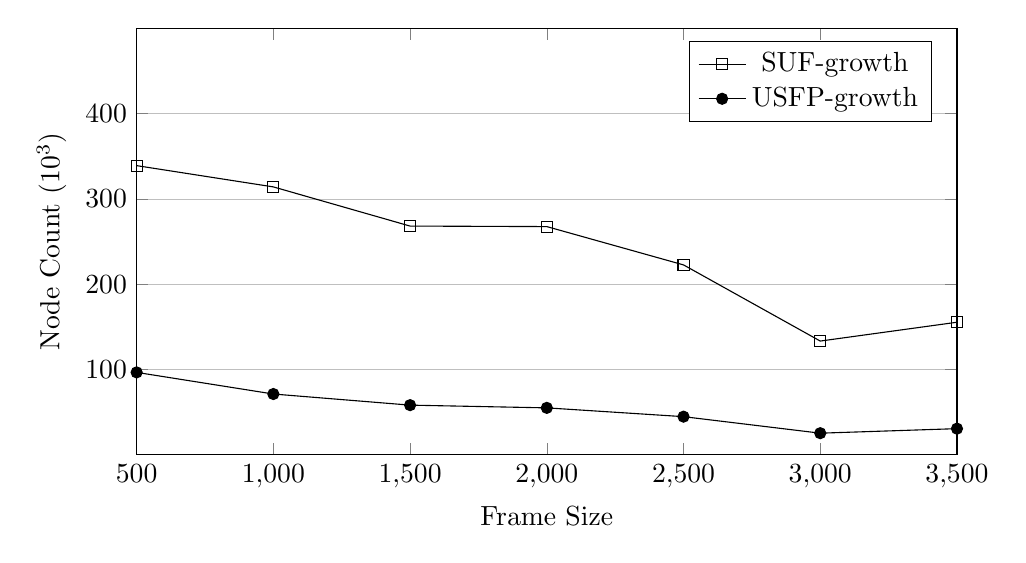
\begin{tikzpicture}
\begin{axis}[
 width=12cm,
   height=7cm,
    xlabel={Frame Size },
    ylabel={Node Count ($10^3$)},
    xmin=500, xmax=3500,
    ymin=0, ymax=500,
    xtick={500,1000,1500,2000,2500,3000,3500},
    ytick={100,200,300,400},
    legend pos=north east,
    ymajorgrids=true,
    grid style={line width=.2pt,draw=gray!50},
]
 
\addplot[
    solid, every mark/.append style={solid, fill=gray}, mark=square
    ]
    coordinates {
			(500,338.966)
			(1000,314.038)
			(1500,268.135)
			(2000,267.525)
			(2500,222.626)
			(3000,133.377)
			(3500,155.435)



	};
    \addlegendentry{SUF-growth}
\addplot[
    solid, every mark/.append style={solid, fill=black}, mark=*
    ]
    coordinates {
			(500,96.670 )
			(1000,71.314)
			(1500,58.275)
			(2000,55.086)
			(2500,44.781)
			(3000,25.416)
			(3500,30.727)


};
    \addlegendentry{USFP-growth}
 
\end{axis}
\end{tikzpicture}
\caption{Total Tree Node vs Frame Size \\(Window Size = 2) for T40I10D100K database}
\label{result:mushroom_total_mem_node}
\end{figure}
%\end{document}